% Introduction

\chapter*{Introduction}
\label{intro} % For referencing the chapter elsewhere, use \ref{Chapter1} 

\lhead{Introduction \emph{Presenting the canvas, etc}} % This is for the header on each page - perhaps a shortened title

%----------------------------------------------------------------------------------------

\section{What is a physics simulation?}

\hspace{.5cm} The purpose of this thesis is to present a series of physics simulations, each modeling a specific problem of physics as realistically as possible.  These simulations differ from \textit{animations}, which can be seen as predictable representations that always display the same visual.  Simulations need to adapt to variable conditions, and be based partly on random processes.    


To program the simulations in this thesis, I chose to write the code in javascript.  This scripting language is easy to view in any modern browser: therefore, all the simulations of this thesis can be viewed online.  I have put the entire thesis and its simulations on my personal website, which can be found at:  http://www.peterkrieg.com/thesis

Javascript combines seamlessly with HTML5, which is why I mostly decided to use it for this thesis.  The evolution of HTML (HyperText Markup Language) has progressed from simple web documents to complex web applications.  For this thesis, every simulation utilizes the HTML5 \textless canvas\textgreater element, which has been used since around 2011.  The HTML5 canvas API allows programmers to write javascript code that accesses the element and runs visual displays through a web browser  The HTML needed to include a canvas can seen below:



\vspace{1cm}
\setstretch{1}
\begin{lstlisting}[breaklines=true, frame=single, numbers=left, caption= The bare bones code necessary for an HTML document to include the canvas element, label=lst:basichtml]
<!doctype html>
<html>
 <body>
  <canvas id="canvas" width="500" height="500" >  
 </body>
 <script>
  var canvas = document.getElementById('canvas');
  var context = canvas.getContext('2d');
 </script>
</html>

\end{lstlisting}
\setstretch{2}

The above code displays the most basic HTML combined with javascript necessary to begin any simulation.  Lines 7-8 are the only ones that actually contain javascript: this is the simple step necessary for the canvas API to recognize the HTML document.  All web browsers include some form of javascript interpreter: whenever the browser encounters a \textless script \textgreater element, it \" passes \" the code onto the JS 












\begin{figure}[h]
	\centering
		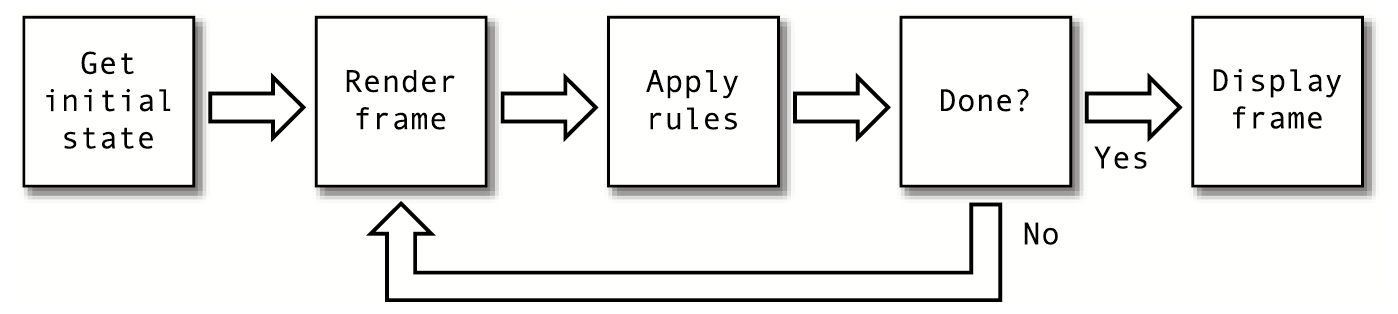
\includegraphics[width=15cm]{Figures/frames.png}

	\caption{The frames of a general simulation}
	\label{fig:frames}
\end{figure}




















%----------------------------------------------------------------------------------------

\section{Learning \LaTeX{}}

\LaTeX{} is not a WYSIWYG (What You See is What You Get) program, unlike word processors such as Microsoft Word or Apple's Pages. Instead, a document written for \LaTeX{} is actually a simple, plain text file that contains \emph{no formatting}. You tell \LaTeX{} how you want the formatting in the finished document by writing in simple commands amongst the text, for example, if I want to use \textit{italic text for emphasis}, I write the `$\backslash$\texttt{textit}\{\}' command and put the text I want in italics in between the curly braces. This means that \LaTeX{} is a ``mark-up'' language, very much like HTML.

\subsection{A (not so short) Introduction to \LaTeX{}}

If you are new to \LaTeX{}, there is a very good eBook -- freely available online as a PDF file -- called, ``The Not So Short Introduction to \LaTeX{}''. The book's title is typically shortened to just ``lshort''. You can download the latest version (as it is occasionally updated) from here:\\
\href{http://www.ctan.org/tex-archive/info/lshort/english/lshort.pdf}{\texttt{http://www.ctan.org/tex-archive/info/lshort/english/lshort.pdf}}

It is also available in several other languages. Find yours from the list on this page:\\
\href{http://www.ctan.org/tex-archive/info/lshort/}{\texttt{http://www.ctan.org/tex-archive/info/lshort/}}

It is recommended to take a little time out to learn how to use \LaTeX{} by creating several, small `test' documents. Making the effort now means you're not stuck learning the system when what you \emph{really} need to be doing is writing your thesis.

\subsection{A Short Math Guide for \LaTeX{}}

If you are writing a technical or mathematical thesis, then you may want to read the document by the AMS (American Mathematical Society) called, ``A Short Math Guide for \LaTeX{}''. It can be found online here:\\
\href{http://www.ams.org/tex/amslatex.html}{\texttt{http://www.ams.org/tex/amslatex.html}}\\
under the ``Additional Documentation'' section towards the bottom of the page.

\subsection{Common \LaTeX{} Math Symbols}
There are a multitude of mathematical symbols available for \LaTeX{} and it would take a great effort to learn the commands for them all. The most common ones you are likely to use are shown on this page:\\
\href{http://www.sunilpatel.co.uk/latexsymbols.html}{\texttt{http://www.sunilpatel.co.uk/latexsymbols.html}}

You can use this page as a reference or crib sheet, the symbols are rendered as large, high quality images so you can quickly find the \LaTeX{} command for the symbol you need.

\subsection{\LaTeX{} on a Mac}
 
The \LaTeX{} package is available for many systems including Windows, Linux and Mac OS X. The package for OS X is called MacTeX and it contains all the applications you need -- bundled together and pre-customised -- for a fully working \LaTeX{} environment and workflow.
 
MacTeX includes a dedicated \LaTeX{} IDE (Integrated Development Environment) called ``TeXShop'' for writing your `\texttt{.tex}' files and ``BibDesk'': a program to manage your references and create your bibliography section just as easily as managing songs and creating playlists in iTunes.

%----------------------------------------------------------------------------------------

